\documentclass[12pt,titlepage]{article}
\usepackage[utf8]{inputenc}
\usepackage[T1]{fontenc}
\usepackage[english]{babel}
\usepackage[a4paper]{geometry}
\frenchspacing
\usepackage{amsfonts}
\usepackage{amsmath}
\usepackage{amssymb}
\usepackage{amsthm}
\usepackage{setspace}
\usepackage{fullpage}
\usepackage{tocbibind}
\usepackage{graphicx}
\usepackage{url}
\usepackage{verbatim}
\usepackage{listings}
%\usepackage{gitinfo2}
\usepackage{hyperref}
\usepackage{cleveref}
\usepackage{cite}
\usepackage{color}
\usepackage{enumitem}
\usepackage{usecases}
\usepackage{nameref}

\definecolor{pblue}{rgb}{0.13,0.13,1}
\definecolor{pgreen}{rgb}{0,0.5,0}
\definecolor{pred}{rgb}{0.9,0,0}
\definecolor{pgrey}{rgb}{0.46,0.45,0.48}
\lstset{language=Java,
  showspaces=false,
  showtabs=false,
  breaklines=true,
  showstringspaces=false,
  breakatwhitespace=true,
  commentstyle=\color{pgreen},
  keywordstyle=\color{pblue},
  stringstyle=\color{pred},
  basicstyle=\ttfamily,
  moredelim=[il][\textcolor{pgrey}]{$$},
  moredelim=[is][\textcolor{pgrey}]{\%\%}{\%\%}
}
\renewcommand{\labelitemi}{$\bullet$}
\renewcommand{\labelitemii}{$\cdot$}
\renewcommand{\labelitemiii}{$\diamond$}
\renewcommand{\labelitemiv}{$\ast$}


\begin{document}
\title{
	Design Document for Bicycle Garage Pro\\
	(Group 33, 2015)\\
	\vspace{0.2in}
	\normalsize Current version: 0.9.1
}
\author{
	Alexander Skafte\\
	\url{tfy13ask@student.lu.se}\\
	Dennis Jin\\
	\url{desuvader@gmail.com}\\
	Petter Berntsson\\
	\url{dat14pbe@student.lu.se}\\
	Emelie Löthman\\
	\url{pol14elo@student.lu.se}\\
	Adam Mzrozek\\
	\url{dat14amr@student.lu.se}
}
\date{}



\maketitle
\newpage
\tableofcontents
\thispagestyle{empty}
\setcounter{page}{0}
\newpage

% ----- REFERENCES & -----------------------------------------------------------
% ----- BIBLIOGRAPHY -----------------------------------------------------------

\section{References}
\label{sec:references}

\begin{itemize}
	\item \textit{Examples and Exercises in the Software
		Engineering Process}. ETSA01 VT 2015. Deparment of Computer
		Science, Lund University. March 10, 2015.
	\item \textit{Requirements Specification for Bicycle Garage
		Pro}. ETSA01, Group 33, 2015.
	\item \textit{Test Plan for Bicycle Garage Pro}. ETSA01, Group 33, 2015.
\end{itemize}

% ----- INTRODUCTION -----------------------------------------------------------

\section{Introduction}
\label{sec:introduction}

\subsection{Purpose}
\label{subsec:introduction-purpose}

This document describes the design of the \textit{Bicycle Garage Pro} software.

The intended audience of this document is primarily the developers responsible
for producing and maintaining the software. The document's purpose is to act as
a guideline during development.

\subsection{Glossary}
\label{subsec:introduction-glossary}
See section 1.2 in the Requirement Specification for Bicycle Garage Pro

\subsection{Scope}
\label{subsec:introduction-scope}

This document is intented to be read in combination with the project's
\textit{Requirements Specification} and \textit{Test plan}, both
referred to in \textit{section \ref{sec:references}: \nameref{sec:references}}.


% ----- ARCHITECTURAL OVERVIEW -------------------------------------------------

\section{Software design overview}

The entire software shall be able to be packaged into a JAR file to be run on a
JVM installed on the main computer in the BGP system. Therefore, the software
shall be written in a JVM-compatible language such as Java, Clojure or Scala.
This particular document describes the software as written in the Java language;
the rationale for this being that Java is an easily accessible and widely known
language. The software thus becomes easy to distribute among BGP systems across
the world.

\subsection{Detailed system description}
\label{sec:detailed-system-description}

See \cref{fig:lol} under \cref{app:example-appendix-section} for the UML diagram that describes the relations between the internal software classes.

\subsection{Modules or Java \texttt{package}s}

This section describes the different modules, organized by Java
\texttt{package}s, that compose the BGP software.

\subsubsection{\texttt{bicyclegarage}}

Below are the classes found in \texttt{package bicyclegarage}.

\begin{description}[font=\normalfont]
	\item [\texttt{Bicycle}]	\hfill \\
		Describes a bicycle owned by a user.

	\item [\texttt{User}]		\hfill \\
		Describes a cyclist using the BGP system.

	\item [\texttt{UserDB}]		\hfill \\
		Mainly handles database saving/loading

	\item [\texttt{Garage}]		\hfill \\
		Ties classes together. Contains the GUI.

	\item [\texttt{Manager}]	\hfill \\
		Mainly implements the methods needed to make the garage work

\end{description}

% May be useful somewhere, so keep it here, but commented out:
%\rule{\textwidth}{1pt}

\subsubsection{\texttt{interfaces}}
Contains the hardware interfaces. Not within this project scope, but still mentioned for convinience sake.
\subsubsection{\texttt{testdrivers}}
Hardware implementations. Not within this project scope, but still mentioned for convinience sake.


% ----- APPENDIX ---------------------------------------------------------------

\newpage
\appendix

\section{UML diagram}
\label{app:example-appendix-section}
\begin{figure}[!h]
\centering
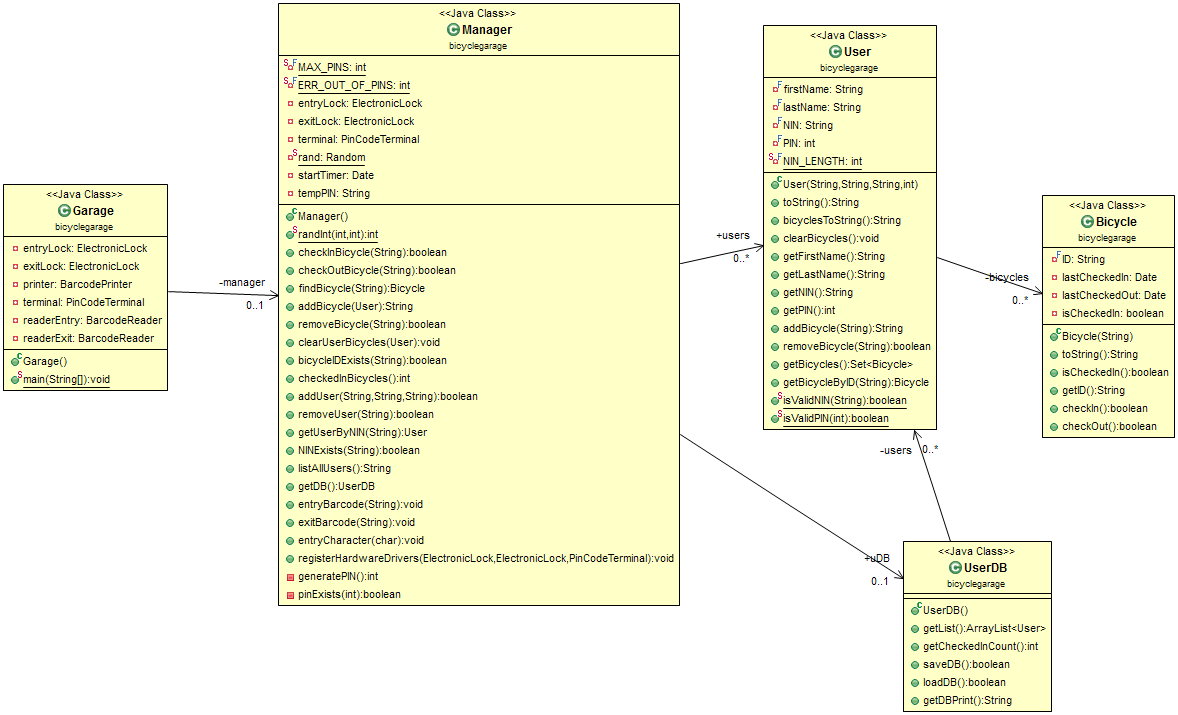
\includegraphics[width=\textwidth]{BGP.png}
\caption{UML diagram for Bicycle Garage Pro (zoomable)}
\label{fig:lol}
\end{figure}
\end{document}

